\subsection{Discretization}

A FE based mesh input is used by Peridigm. As it is expected there are differences in the choice of the horizon and element size for structured and unstructured based meshes, both are considered here. The specimen creation in a versatile parametric model generator allows for a quick change of the underlying discretization scheme and the element size. The base FE models and resulting PD discretizations are shown in \autoref{fig:Model:Discretization}.


% Styles
\tikzset{
  modelspy style/.style={
    spy scope={%
      modelspyscope style,%
    },
    connect spies/.style={
      modelspyconnect style,%
    },
  }
}

\tikzset{
  modelspyscope style/.style={
    magnification=4,
    connect spies,                            % Connect orig. & detail
    width=0.3\linewidth,                      % Spy width
    height=0.2\linewidth,                    % Spy height
    every spy on node/.style={                % Source
      rectangle,                              % Form
      rounded corners=0.01\linewidth,         % Edge shape
      dashed,                                 % Dashed line
      draw=black,                             % Line color
      %thick,                                  % Line style for spy
    },
    every spy in node/.style={                % Spy
      rectangle,                              % Form
      rounded corners=0.04\linewidth,         % Edge shape
      dashed,                                 % Dashed line
      draw=black,                             % Line color
      %thick,                                  % Line style for spy
    },
  },
}

\tikzset{
  modelspyconnect style/.style={
    spy connection path={
      \draw[%
        %thick,
        dashed,
        black
      ] (tikzspyonnode) -- (tikzspyinnode); % In-On-Connection
    },
  },
}
% Hex:
\begin{figure}[htbp]
  \begin{subfigure}{0.49\linewidth}
    \centering
    %\includegraphics[width=\linewidth,height=4cm,keepaspectratio]{../../Material/Figures/Model_FE_Hex_0-4_ct}
    %\includegraphics[width=\linewidth,height=4cm,keepaspectratio]{Model_FE_Hex_0-4_ct}
    \tikzexternalenable
    \tikzsetnextfilename{Model_FE_Hex_0-4_ct}
    \begin{tikzpicture}[modelspy style]
      \node[anchor=south west,inner sep=0] (image) at (0,0) {\includegraphics[width=\linewidth,height=4cm,keepaspectratio]{Model_FE_Hex_0-4_ct}};
      \begin{scope}[
        shift={(image.south west)},
        x={(image.south east)},
        y={(image.north west)},
      ]
        \coordinate (spypointfehex) at (0.825,0.740);
        \coordinate (spyviewerfehex) at (0.80,0.25);
        \spy on (spypointfehex) in node at (spyviewerfehex);
      \end{scope}
    \end{tikzpicture}
    \tikzexternaldisable
    \caption{Base hex FE mesh}
    \label{fig:Model:Discretization:Hex:FE}
  \end{subfigure}%
  \hfill
  \begin{subfigure}{0.49\linewidth}
    \centering
    %\includegraphics[width=\linewidth,height=4cm,keepaspectratio]{../../Material/Figures/Model_PD_Hex_0-4_ct}
    %\includegraphics[width=\linewidth,height=4cm,keepaspectratio]{Model_PD_Hex_0-4_ct}
    \tikzexternalenable
    \tikzsetnextfilename{Model_PD_Hex_0-4_ct}
    \begin{tikzpicture}[modelspy style]
      \node[anchor=south west,inner sep=0] (image) at (0,0) {\includegraphics[width=\linewidth,height=4cm,keepaspectratio]{Model_PD_Hex_0-4_ct}};
      \begin{scope}[
        shift={(image.south west)},
        x={(image.south east)},
        y={(image.north west)},
      ]
        \coordinate (spypointpdhex) at (0.825,0.740);
        \coordinate (spyviewerpdhex) at (0.80,0.25);
        \spy on (spypointpdhex) in node at (spyviewerpdhex);
      \end{scope}
    \end{tikzpicture}
    \tikzexternaldisable
    \caption{PD representation of hex mesh}
    \label{fig:Model:Discretization:Hex:PD}
  \end{subfigure}%
  \\
%   \caption{Structured discretization}
%   \label{fig:Model:Discretization:Hex}
% \end{figure}
% 
% Tet:
% 
% \begin{figure}[htbp]
  \begin{subfigure}{0.49\linewidth}
    \centering
    %\includegraphics[width=\linewidth,height=4cm,keepaspectratio]{../../Material/Figures/Model_FE_Tet_0-67_ct}
    %\includegraphics[width=\linewidth,height=4cm,keepaspectratio]{Model_FE_Tet_0-67_ct}
    \tikzexternalenable
    \tikzsetnextfilename{Model_FE_Tet_0-67_ct}
    \begin{tikzpicture}[modelspy style]
      \node[anchor=south west,inner sep=0] (image) at (0,0) {\includegraphics[width=\linewidth,height=4cm,keepaspectratio]{Model_FE_Tet_0-67_ct}};
      \begin{scope}[
        shift={(image.south west)},
        x={(image.south east)},
        y={(image.north west)},
      ]
        \coordinate (spypointfetet) at (0.825,0.740);
        \coordinate (spyviewerfetet) at (0.80,0.25);
        \spy on (spypointfetet) in node at (spyviewerfetet);
      \end{scope}
    \end{tikzpicture}
    \tikzexternaldisable
    \caption{Base tet FE mesh}
    \label{fig:Model:Discretization:Tet:FE}
  \end{subfigure}%
  \hfill
  \begin{subfigure}{0.49\linewidth}
    \centering
    %\includegraphics[width=\linewidth,height=4cm,keepaspectratio]{../../Material/Figures/Model_PD_Tet_0-67_ct}
    %\includegraphics[width=\linewidth,height=4cm,keepaspectratio]{Model_PD_Tet_0-67_ct}
    \tikzexternalenable
    \tikzsetnextfilename{Model_PD_Tet_0-67_ct}
    \begin{tikzpicture}[modelspy style]
      \node[anchor=south west,inner sep=0] (image) at (0,0) {\includegraphics[width=\linewidth,height=4cm,keepaspectratio]{Model_PD_Tet_0-67_ct}};
      \begin{scope}[
        shift={(image.south west)},
        x={(image.south east)},
        y={(image.north west)},
      ]
        \coordinate (spypointpdtet) at (0.825,0.740);
        \coordinate (spyviewerpdtet) at (0.80,0.25);
        \spy on (spypointpdtet) in node at (spyviewerpdtet);
      \end{scope}
    \end{tikzpicture}
    \tikzexternaldisable
    \caption{PD representation of tet mesh}
    \label{fig:Model:Discretization:Tet:PD}
  \end{subfigure}%
%   \caption{Unstructured discretization}
%   \label{fig:Model:Discretization:Tet}
  \caption{Discretization schemes and PD representation}
  \label{fig:Model:Discretization}
\end{figure}

The structured mesh is doubly symmetric regarding the specimen $x$-$y$- as well as the $x$-$z$-plane. The unstructured meshes are only symmetric about the $x$-$z$-plane.

Especially in higher dimensions, the horizon cannot be too large either as this results in the boundary layer, where displacement boundary conditions are imposed, being the majority of the simulation domain \cite{SelesonP2016b}. Thus, a no-damage zone (red) is introduced in the vicinity of the specimen ends. In this region failure is not modeled to avoid effects of the boundary conditions on the failure behavior. Based on the findings in the experiments this approach is valid.


